%!TEX TS-program = xelatex
%!TEX root = ../../maxwell2018thesis.tex

\chapter{Introduction}\label{chap:intro}
We live today in the so-called \emph{Information Age}, an era of human history characterised by the rapid development of technology allowing for the creation, transmission and retrieval of large volumes of information. Two key developments that have permitted such an increase in information generation are the electronic computer and the associated technologies that allow for near-instantaneous communications with devices all around the planet, including the \emph{Internet} and~\gls{acr:www}~\citep{berners1994www}. Indeed, with such technologies now ubiquitous in today's society, we collectively generate something in the range of \emph{2.5 quintillion bytes} \emph{per day}\footnote{$2.5$ quintillion bytes = $2,500,000,000,000,000,000$ bytes, or $2,500,000$ terabytes. This means that every day, enough data is generated to fill the \emph{US Library of Congress} 250,000 times over.}, according to a recent \emph{IBM} technical report\footnote{\url{https://www-01.ibm.com/common/ssi/cgi-bin/ssialias?htmlfid=WRL12345USEN}\urlaccessed{2017-11-23}}.

%  To use a different unit of measurement, 250,000 times the amount of information held at the \emph{US Library of Congress}\footnote{This is calculated using the approximation on the US Library of Congress Blog, that says the Library holds the equivalent of 10 terabytes of information.}.

\begin{figure}[h]
    \centering
    \vspace{5mm}
    \resizebox{1\hsize}{!}{
    
\includegraphics{figures/ch1-earth.pdf}}
    \label{fig:stopsign}
    \vspace{-4mm}
\end{figure}

Sifting through such large volumes of information online to find the elusive and proverbial \emph{needle in the haystack} has been an area of active research and development over a number of decades. Since the early 1990's, the~\gls{acr:www} has emerged as the dominant means of publishing information online over the Internet, replacing obsolete technologies such as the \emph{Gopher} protocol.\footnote{Gopher was designed primarily with a menu-driven interface in mind (i.e. selecting options from a series of choices). The Gopher ecosystem provided the foundations for the~\gls{acr:http} protocol, which the~\gls{acr:www} today utilises.}. As the amount of information available on the~\gls{acr:www} grew\footnote{According to \url{http://www.internetlivestats.com/total-number-of-websites/}, September 2014 saw the point at which 1 billion unique websites were present on the~\gls{acr:www}.\urlaccessed{2018-05-21}}, so too did the paradigms that were employed by those wishing to seek information on it.

Over the course of the \emph{noughties}, the approach demonstrated by \emph{information seekers} for finding information online changed from the concept of \emph{surfing} a particular domain by following a series of set~\glspl{glos:hyperlink} within documents, to explicitly \blueboxbold{searching} the ever increasing universe of documents available at their disposal (refer to Figure~\ref{fig:ch1-surfing}).\footnote{Indeed,~\cite{mcbryan1994taming_tools} considered a search engine as a means of \emph{taming} the considerable number of documents online.} This is not to say that surfing no longer occurs; procrastinators (the author included...) might find solace by surfing the myriad of content available on \emph{Reddit,} billed as the \emph{``front page of the Internet''}\footnote{\url{https://www.reddit.com}\urlaccessed{2018-05-21}}. However, for a task where an individual has a specific \emph{information need,} searching become by far the most dominant paradigm for seeking required information. As such, the development of effective \emph{search engines} has been of paramount importance, with the development of search engines seen as the \emph{raison d'\^{e}tre} of the study of~\gls{acr:ir}.

\begin{figure}[t!]
    \centering
    \resizebox{1\hsize}{!}{
    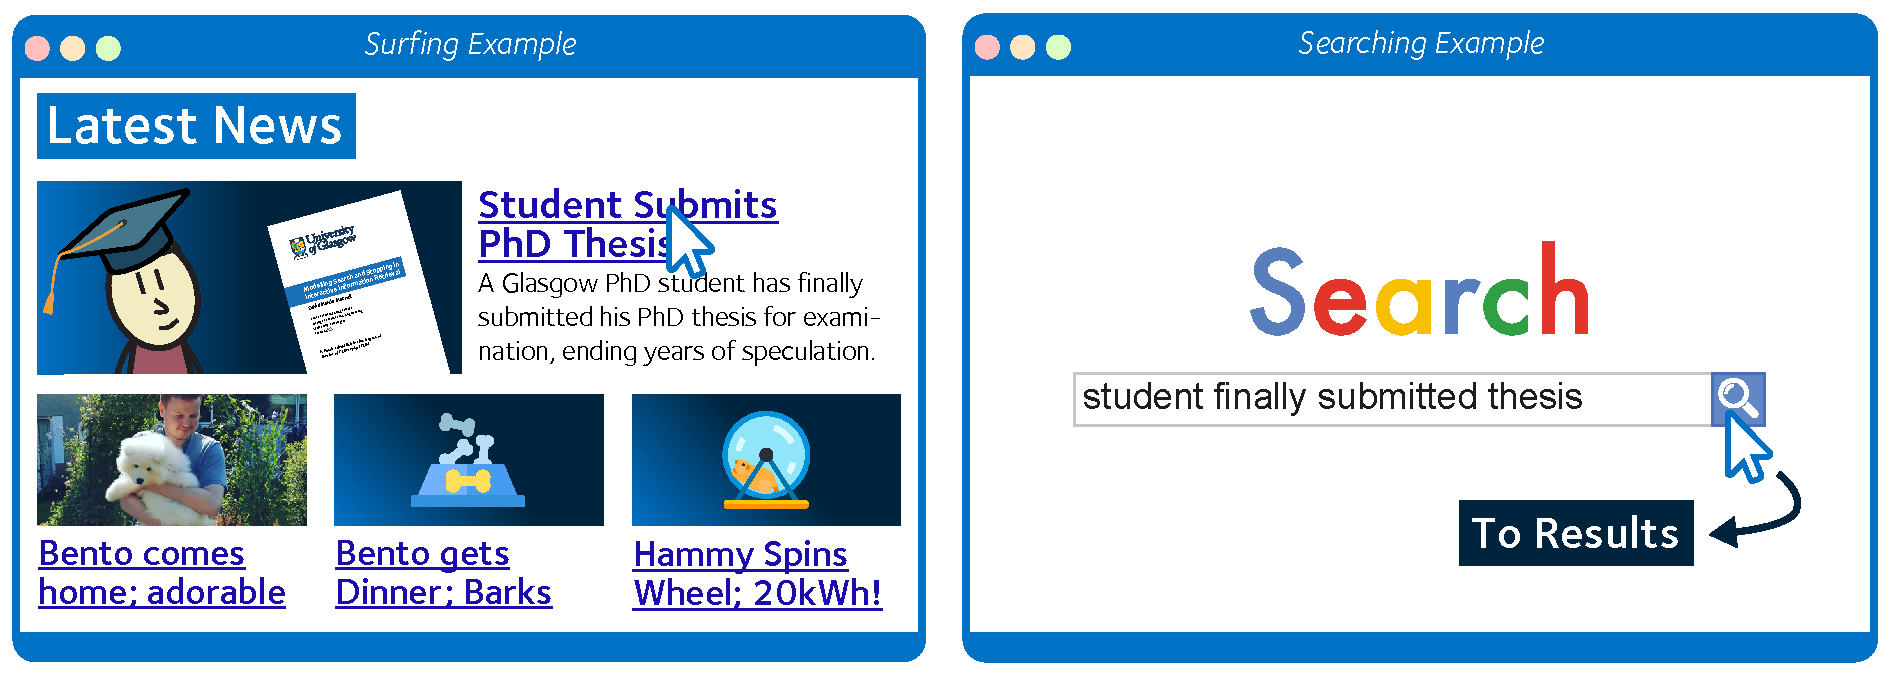
\includegraphics{figures/ch1-surfing.pdf}}
    \caption[Surfing vs. Searching]{The paradigms of surfing and searching. On the left, a seeker will navigate through a series of documents via~\glspl{glos:hyperlink} (perhaps without a specific \emph{information need} in mind), while a searcher (right) will issue a \emph{query} articulating their information need, relying on an underlying \emph{search engine} to \emph{retrieve} documents that it thinks will assist the seeker.}
    \label{fig:ch1-surfing}
\end{figure}

\begin{quote}
    \emph{``...but perhaps the key technology that took the web from a useful supplement of current information practice to become the default communication medium is search.''}
    \attrib{\cite{wilson2010keyword_search}}
\end{quote}

Contemporary search engines such as \emph{Google} and \emph{Bing} are considered to offer an effective means of finding the proverbial needle in the haystack~\citep{wilson2010keyword_search}, where near perfect accuracy is regularly attained for popular \emph{queries}~\citep{vaughan2004new_measurements}. These search engines, along with the many others in existence today under a variety of different contexts\footnote{Google and Bing may be the most popular search engines for \emph{general web queries,} but other contexts can include patent search, enterprise search and multimedia search, as examples.}, are the product of the collective work undertaken in the field of~\gls{acr:ir} -- from early research in the 1970's~\citep{cleverdon1962cranfield_experiments,rijsbergen1979ir}; to the development of various \emph{retrieval models}~\citep{robertson2009probabilistic_models}; to the setting up of \emph{evaluation forums}~\citep{harman1993trec1}; to the development of the \emph{large-scale search engines} (or \emph{retrieval systems}) that are commonplace today~\citep{baezayates1999modern_ir, wang2010language_models}.

The work that the field of~\gls{acr:ir} collectively undertakes is all done in the interests of making it easier for potential users of search engines to satisfy their underlying \emph{information need}. Armed with a preexisting knowledge of the world, an individual will develop an information need from a perceived problem -- either from a knowledge gap, an internal consistency, or a conflict of evidence. This state has been referred to as the \emph{anomalous state of knowledge}~\citep{belkin1980ask}. A searcher then formulates a \emph{query} -- an expression of what they are looking for~\citep{borlund2003iir_model}, typically consisting of a number of different terms -- before being presented with a potentially relevant set of documents. From this set of documents, an individual can then begin the process of examining them for relevance. A number of complex interactions take place between an individual seeking information and the search engine that is being utilised~\citep{ingwersen2005theturn}. This process, where the searcher engages in \emph{dialogue} with the search system, is considered the study of~\glsfirst{acr:iir}~\citep{borlund2003iir_model}. As such, work has been undertaken that attempts to help us better understand these complex interactions, and potentially assist in making the search process a more seamless experience.

\section{Motivation and Context}\label{sec:intro:motivation}
Central to much of the work undertaken in the field of~\gls{acr:ir} over the past 50 years is the so-called \emph{Cranfield paradigm}, a term denoting a standardised approach for the \emph{evaluation} of~\gls{acr:ir} systems. The Cranfield paradigm descends directly from \emph{Cranfield II}~\citep{aslib1966factors}, a set of experiments designed to evaluate the efficiency of \emph{indexing systems}\footnote{The process of indexing, as discussed later in Section~\ref{sec:ir_background:basics:indexing}, involves turning a number of source documents into a form of data structure that can be traversed, or \emph{searched,} in a quick and efficient manner.}. At the time, searching for information on computer systems was achieved through the issuance of queries to a \emph{boolean retrieval system} (refer to Section~\ref{sec:ir_background:basics:models:boolean}), with terms matched against a small set of manually indexed documents~\citep{harman2010cranfield}. Results were compared against a set of \emph{a priori} \emph{relevance judgements} for each of the documents, as judged by humans, allowing one to then ascertain the performance of a given retrieval system.
%We discuss this high-level approach in Section~\ref{sec:ir_background:basics:cranfield}.

While the basic principles of the Cranfield paradigm have remained in place since it was established in the 1960's, components of the approach have evolved over the years to cater for the ever increasing complexity of the tasks at hand~\citep{harman2010cranfield}. Indeed, the approach is still widely used in evaluation forums, such as the~\gls{acr:nist} sponsored~\gls{acr:trec} -- the first of which was held in 1993~\citep{harman1993trec1}. Indeed, many of the relevance judgements and \emph{topics} (i.e. information needs) provided as part of \emph{\gls{acr:trec} Tracks} over a number of years are used as ground truths throughout the work discussed in this thesis.

This approach however can be argued to remain simplistic in terms of consideration of the complex user interactions that take place during the search process~\citep{borlund2000evaluation_iir,ingwersen2005theturn}. In other words, the Cranfield paradigm broadly fails to consider the complexities of the~\gls{acr:iir} process, where, for example, searchers can issue multiple queries during the course of a search session, and adapt their interactions based upon the perceived quality of the presented ranked list of results for each associated query~\citep{moffat2013users_versus_models}. Selecting good terms to use within a query is difficult yet important~\citep{efthimiadis2000query_expansion}; as such, the initial query posed in a search session often acts as an entry to the search system, followed by phases of browsing and query reformulations~\citep{marchionini1993information_seeking}.

Searchers also will typically abide by the principle of least effort, whereby they strive to minimise the probable average rate of work expenditure over time~\citep{zipf1949behaviour}. Cranfield makes a series of assumptions, namely that that a user will: \emph{(i)} issue a single query; \emph{(ii)} examine documents to a great depth (typically $1,000$ documents); and \emph{(iii)} consider all documents to be relevant. This is largely unrealistic, and numerous researchers have proposed alternatives to the Cranfield paradigm --~\cite{borlund2003iir_model}, for example.

Considering alternatives to the Cranfield paradigm,~\cite{keskustalo2008user_simulation} categorised~\gls{acr:iir} research into four different approaches that allow for the consideration of the complex interactions that take place between a human and the search engine being used. The four approaches, as illustrated in Figure~\ref{fig:ch1-options}, can themselves be divided into two categories. The first category considers approaches that utilise \blueboxbold{real-world searchers}, namely:

\begin{itemize}
    \item[]{\blueboxbold{1} the \blueboxbold{observation of real-world searchers} in real world scenarios (e.g. general web search), through the use of \emph{interaction logs;} and}
    \item[]{\blueboxbold{2} the observation of \blueboxbold{real-world searchers undertaking simulated work tasks} in a lab-based environment (i.e. a \emph{user study}).}
\end{itemize}

The final two options \emph{do not explicitly} consider real-world searchers, but rather aim to mimic their behaviours. These approaches are:

\begin{itemize}
    \item[]{\blueboxbold{3} performing \blueboxbold{simulations of interaction} in a lab-based environment, \emph{sans} real-world searchers; and of course}
    \item[]{\blueboxbold{4} the undertaking of \blueboxbold{traditional, Cranfield style lab-based experimentation}.}
\end{itemize}

\begin{figure}[t!]
    \centering
    \resizebox{1\hsize}{!}{
    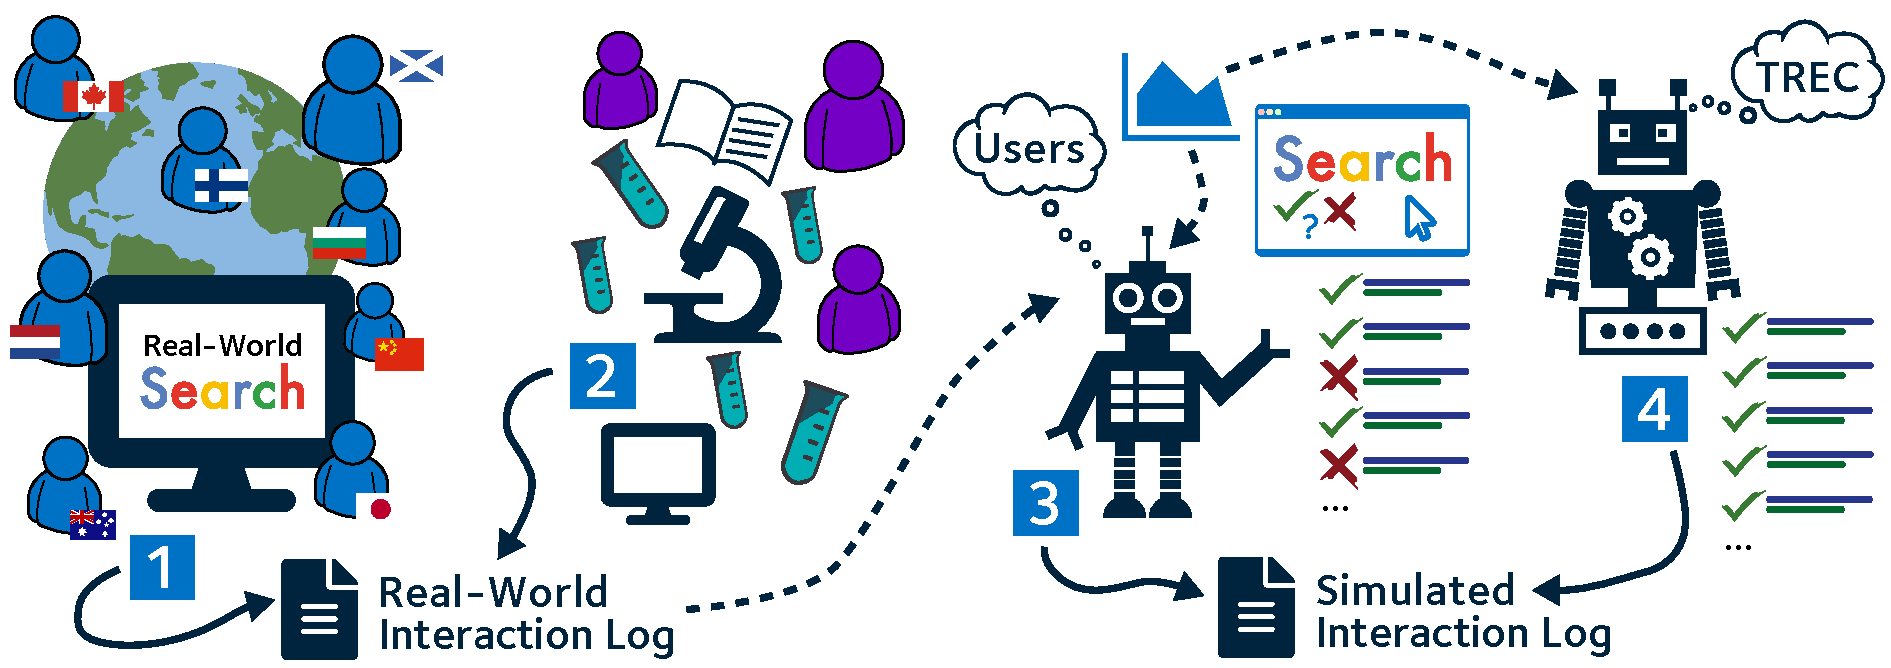
\includegraphics{figures/ch1-options.pdf}}
    \caption[Approaches to~\gls{acr:iir} research]{The four approaches for~\gls{acr:iir} research, as outlined by~\cite{keskustalo2008user_simulation}. Detailed in Section~\ref{sec:intro:motivation}, approaches \blueboxbold{1} \emph{(real-world)} and \blueboxbold{2} \emph{(user studies)} consider log data from real-world searchers, with options \blueboxbold{3} \emph{(simulations of interaction)} and \blueboxbold{4} \emph{(traditional experimentation)} considering log data as generated from \emph{simulations.} Note the \emph{grounding} (dashed line) of log data from either approach \blueboxbold{1} or \blueboxbold{2} to complement approach \blueboxbold{3} (refer to Section~\ref{sec:intro:simulation}).\vspace*{10mm}}
    \label{fig:ch1-options}
\end{figure}

Obtaining interaction data from studies utilising real-world users undertaking search tasks (categories \blueboxbold{1} and \blueboxbold{2}) will of course always be the preferred option. There can never be a better substitute than examining the real thing. However, there are pitfalls with both approaches that must be considered, primarily in terms of \emph{availability} and \emph{cost}. Obtaining data for studies conducted in category \blueboxbold{1} is difficult if the researchers do not work for an organisation offering a large-scale search engine, such as \emph{Google} or \emph{Microsoft.} Working within an academic setting for example may greatly restrict what data can be obtained. Indeed, working with real-world interaction data also leads to major ethical and privacy concerns~\citep{korolova2009aol_query_log_privacy}. The release of the \emph{AOL Query Log} (and subsequent fallout) in August 2006 is testament to that, although this has not stopped researchers from utilising the data in their work (refer to~\cite{brenes2009aol_query_log} for such an example).

This will leave many researchers with category \blueboxbold{2} -- especially those in a non-industrial setting. While this approach also leads to the capturing of real-world interaction data, pitfalls of this approach primarily are the significant costs involved in such an approach -- both financially and in terms of time. Considerations must also be placed into study design to mitigate potential biases. In recent years however, the concept of \emph{crowdsourcing} may alleviate some of these concerns, and open up a potential study to a larger potential audience. A recent study has shown that using crowdsourcing to capture interaction data is no worse than a carefully controlled lab-based user study~\citep{zuccon2013crowdsourcing_comparisons}, although quality control measures must be taken.

While categories \blueboxbold{1} and \blueboxbold{2} provide real-world interaction data, options \blueboxbold{3} and \blueboxbold{4} do not. Such approaches however, if executed correctly, can potentially lead to insights that would not otherwise be possible when involving real-world users. As an example, covering an extensive set of test cases with real-world searchers may simply not be possible~\citep{keskustalo2008user_simulation} -- perhaps due to financial constraints, or a lack of suitable subjects. Category \blueboxbold{4} can be considered as a means of conducting \emph{traditional, TREC-style}~\gls{acr:ir} lab experimentation that is, as previously mentioned, largely na\"{i}ve of the user's complex interactions. This leaves category \blueboxbold{3} as a means of conducting and evaluating user-sided experimentation without the explicit need for real-world users to be present. \blueboxbold{Simulation} is used as a means to conducting such experiments.

\subsection{Considering Simulation}\label{sec:intro:simulation}
Simulation is defined as the \emph{imitation of the operation of a real-world process or system over time}~\citep{banks1996discrete}. Such an approach allows one to gain insight into the functioning of some real-world phenomenon. Simulation has been used in a wide range of areas, including, for example, examining physical processes~\citep{haessig1991physics_modelling}, psychology~\citep{hastie1988human_memory_simulation}, road traffic~\citep{mahmud2016traffic_modelling_electric} and training for various activities, such as piloting an aeroplane~\citep{sparko2010flight_simulators}. Central to contemporary uses of simulation is the idea of \emph{computerised simulation}~\citep{heermann1990computer_simulation}. Thanks to ever increasing computational power in~\glspl{acr:cpu} and~\glspl{acr:gpu} available for such tasks, such as the simulation of racing cars for the purposes of driver development, as shown in Figure~\ref{fig:ch1-mclaren}. With computer simulation, a real-world object can be imitated with varying degrees of realism. Alternatively, individual components that comprise a larger system can be examined and simulated in isolation, allowing researchers to obtain a more detailed understanding of how individual components react to changes in their environment. As such, simulation can provide a rapid means of exploring aspects of a real-world phenomenon, all at a low cost -- all the while permitting repeatable, and therefore reproducible, results~\citep{maxwell2016agents}.

\begin{figure}[t!]
    \centering
    \resizebox{1\hsize}{!}{
    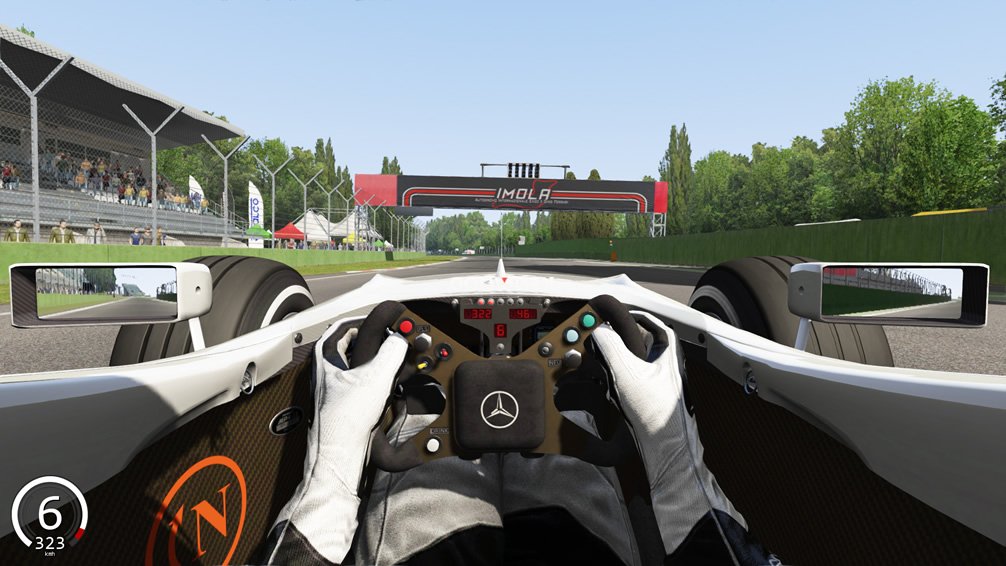
\includegraphics{figures/ch1-mclaren.jpg}}
    \caption[Racing Simulator Example]{An example of a \emph{video game simulation}, \emph{Assetto Corsa}. In this illustration is a model of the \emph{McLaren-Mercedes MP4/13} race car (complete with terrible gear ratios), driving around the \emph{Autodromo Enzo e Dino Ferrari} circuit in northeastern Italy. In the past ten years, increases in~\gls{acr:cpu} and~\gls{acr:gpu} performance has enabled the development of increasingly complex (and \emph{more realistic}) video game simulations, which, for example, are now used in the training of racing drivers.}
    \label{fig:ch1-mclaren}
\end{figure}

One of the key components of any simulation -- regardless of whether it is executed on a computer or not -- is that of an underlying \emph{model} of the real-world phenomenon being simulated~\citep{tocher1963art_of_simulation}. This model defines the various stages, rules and other descriptive components of the phenomenon that simulations must consider. These rules are often high level, and as such, a number of \emph{assumptions} are made~\citep{tocher1963art_of_simulation}. For example, the~\gls{acr:trec} model of search (as detailed in Section~\ref{sec:stopping_background:models}) assumes that a single query is issued by a searcher within a search session, and searchers examine to great depths per query. These assumptions should be made in the face of supporting evidence; evidence in~\gls{acr:iir} studies strongly suggests that searchers do not follow this rigid approach, but rather adapt their behaviour based upon cues that are presented to them.

Why though, use simulation when other alternatives to modelling the search process are available? Alternatives include some form of closed-form system, such as a series of linear equations to describe the complex interactions that take place. However, according to~\cite{fishwick1995simulation}, this approach is not flexible enough, and a number of reasons are linked as to why simulation is essential in complex, dynamic systems:

\begin{itemize}
    \item{the model is very complex, with many variables and interacting components;}
    \item{the underlying variables and relationships are non-linear;}
    \item{the underlying models contains random variates; and}
    \item{the model output is to be visual, as in a three-dimensional computer animation.}
\end{itemize}

In the context of~\gls{acr:iir}, the first three reasons can be considered as acceptable reasons for why simulation is an advantageous methodology to pursue. For example, many state-of-the-art~\gls{acr:iir} models consider a stochastic component when determining the relevancy of a document to a particular information need (or~\gls{acr:trec} topic).

Simulation provides a means of using a uniform model execution technique that can be used to solve a large variety of systems, without resorting to a \emph{``bag of tricks'',} where one must choose special purpose and sometimes arcane solutions to avoid simulation~\citep{fishwick1995simulation}. Simulation provides the freedom and flexibility to permit the implementation of a model that better represents the real-world phenomenon that is being considered. In contrast, with a more closed-form approach, the underlying model that is created is often twisted and altered to suite the closed-form approach, rather than to actually represent the real-world system. This leads to a larger gap between the model and reality, and as such leads to a greater number of assumptions within the model than what would otherwise be required. In other words, the technique used to develop the model constrains just how realistic is can be. Simulation provides the freedom and flexibility to reduce assumptions that may otherwise be included.

As a means of testing better and more flexible models of search, simulation has been extensively used within~\gls{acr:ir}. While we provide an overview of simulation of~\gls{acr:ir} in Section~\ref{sec:ir_background:user:simulation}, one such area that has been studied is \emph{simulated interaction,} where one attempts to mimic the behaviours that a searcher exerts when interacting with a search engine -- and is exactly what we consider in this thesis. While this encapsulates category \blueboxbold{3} of the four categories outlined by~\cite{keskustalo2008user_simulation}, we also argue that in order to run simulations of interaction \emph{`correctly',} they must be \emph{grounded} using real-world observations, which in turn means that the assumptions can be considered to be credible abstractions of the real-world phenomenon. As such, this necessitates access to data obtained through either categories \blueboxbold{1} or \blueboxbold{2} -- or, in other words, data from \emph{real-world searchers.} Without access to a large-scale search engine for this research, this leaves category \blueboxbold{2} as a means for acquiring such data, and provides an explanation between the linking of the real-world interaction log, and simulated users (via the dashed line) in Figure~\ref{fig:ch1-options} on page~\pageref{fig:ch1-options}.

\noindent
\blueboxbold{In a Nutshell – Simulation and this Thesis}
Given all of the above, this thesis proposes a more advanced, realistic model of the search process. In line with the suggestions outlined in the work by~\cite{keskustalo2008user_simulation}, simulations of interaction are trialled (category \blueboxbold{3}), with the underlying components of the model \emph{grounded} using interaction data extracted from two different user studies, also conducted as part of this thesis. One particularly important phenomenon that has been largely overlooked in the~\gls{acr:iir} literature is that of a searcher's \blueboxbold{stopping behaviour} (e.g. \emph{given this list of ranked results, how far down the list should I go before I stop?}). In the next section, we provide a brief introduction on why stopping behaviour is important, before considering this thesis' research statement.

\subsection{Considering Stopping Behaviours}\label{sec:intro:stopping}
\begin{wrapfigure}[7]{r}{0.45\textwidth}
    \begin{center}
    \vspace*{-13mm}
    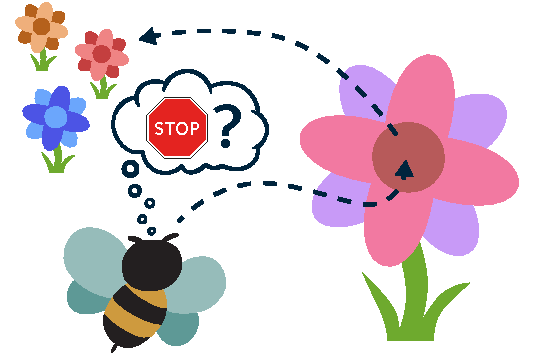
\includegraphics[width=1\textwidth]{figures/ch1-bee.pdf}
    \end{center}
    \vspace*{-4mm}
    \label{fig:bee}
\end{wrapfigure}

With any activity that a creature makes, there has to come a time when it makes a decision to \emph{stop} what it is doing. A honeybee, when collecting pollen on a flowerhead, will eventually stop collecting and fly away to another flower. An exhausted PhD student, when writing his or her thesis, will eventually stop writing for the night once he or she has become too tired -- something the author knows only all too well. Similarly, when applied to the context of search, an individual will also make a decision to eventually stop examining content. These examples demonstrate that knowing when to stop is a fundamental aspect of animal -- and by definition, human -- thinking and behaviour.

But given this, what actually makes us decide when to stop doing something? Obviously, different \emph{external factors} can influence this decision, such as finding no more pollen on a flowerhead, or time pressure that is exerted upon us. Moreover,~\citep{nickles1995judgment} argues that \emph{knowing when to stop} is largely determined by a series of \emph{internally defined, stopping criteria} that the decision maker employs. This makes stopping a phenomenon that is incredibly difficult to model effectively. We discuss this in more detail in Section~\ref{chap:stopping_background:why}.

Given the fact that internal factors are a major drive to determining when to stop, studies have largely been unable to quantify \emph{why} searchers stop, other than what they find gives them the feeling that it is \emph{``good enough''}~\citep{zach2005enough_is_enough}. Researchers have however attempted to create a series of \emph{reasoning} and \emph{judgement} based \blueboxbold{stopping heuristics} that attempt to formally define when a searcher should stop. It is these stopping heuristics that we will primarily consider in this thesis. In conjunction with an updated user model of search, these heuristics can then be integrated into the model, allowing us to determine whether they offer better or worse approximations of actual searcher stopping behaviours.

Examining stopping behaviour during search is important because it considers the judgements of a searcher as part of their interactions. For example, it would be prudent of a searcher examining a list of results that are mostly considered to be non-relevant to a given information need to stop early, and thus save time and effort. In other words, a good stopping heuristic allows a searcher to become \emph{more efficient.} This can be achieved in a number of different places -- or \blueboxbold{stopping decision points} -- during search, such as the depth to which a searcher will examine a list of results.

\section{Overarching Research Questions}\label{sec:intro:rqs}
From the introductory explanations of the problem space above, we can now formulate the four main overarching, high level research questions -- denoted as \blueboxbold{HL-RQ} -- that the work in this thesis addresses. Our first research question considers the concept of user modelling, and how, with an emphasis of examining stopping decision points, we can improve the current model to better reflect actual searcher behaviours.

\begin{itemize}
    \item[]{\blueboxbold{HL-RQ1} How can we improve the current state-of-the-art searcher model to incorporate different points where individuals subscribing to such a model can stop?}
\end{itemize}

As previously stated, being able to improve the current state-of-the-art from a stopping perspective should allow those subscribing to such a model to become more efficient at how they search. Closely related to this advancement in user modelling is the consideration of the various stopping heuristics, as briefly outlined in Section~\ref{sec:intro:stopping}.

\begin{itemize}
    \item[]{\blueboxbold{HL-RQ2} Given the stopping heuristics defined in the literature, how can we encode these heuristics into a series of operationalised, programmable \blueboxbold{stopping strategies} that can be subsequently evaluated?}
\end{itemize}

The heuristics that we detail later in Section~\ref{sec:stopping_background:heuristics} are high level in nature, and no not provide an explanation as to how they can be \emph{operationalised} within a wider system. The challenge that must be addressed in order to answer this question will be how we can operationalise these heuristics within a wider, common framework.

Our final two overarching research questions can be considered similar in nature, and are numbered as such. With a more realistic model of the search process defined by addressing \blueboxbold{HL-RQ1} and a series of stopping strategies defined by addressing \blueboxbold{HL-RQ2}, how well do the combinations of an improved model and different stopping strategies perform?

\begin{itemize}
    \item[]{\blueboxbold{HL-RQ3a} Given these operationalised stopping strategies, how well do simulated searchers using these strategies perform?}
    \item[]{\blueboxbold{HL-RQ3b} How closely do the operationalised stopping strategies compare to the stopping behaviours of real-world searchers?}
\end{itemize}

With the flexibility provided by the approach, simulation is an ideal mechanism for achieving a means to address these two research questions. These questions are of course very broad in nature -- as should be expected for overarching questions -- and it is simply not possible to evaluate them in every conceivable search context. As we discuss in the following section, we will examine these questions in several different contexts which are likely to impact upon the stopping behaviours of searchers.

\section{Thesis Contributions}\label{sec:intro:contribs}
From our four overarching research questions defined above, we identify four major contributions offered by the work presented in this thesis. Listed and detailed below, we consider primary contributions from conceptual, theoretical and empirical standpoints. We also consider the general methodology that we utilise throughout the work in this thesis.

\noindent
\blueboxbold{Conceptual Model}
Our first contribution is that of a searcher model. Taking the current state-of-the-art, we propose an updated, high-level model of the search process. We call this model the \blueboxbold{\gls{acr:csm}}, and this provides us with a solution for addressing \blueboxbold{HL-RQ1}. Outlined in Section~\ref{sec:csm:csm}, the conceptual~\gls{acr:csm} outlines a series of different activities and decision points that searchers undertake throughout the search process, and establishes a flow of interaction based upon established models. Within the~\gls{acr:csm} are a number of innovations, central to the work in this being a new stopping decision point. Combined together, these improvements allow us to ascertain a better understanding of the search process, and the complex interactions between a searcher and search system that take place. Being a conceptual model, we can take the~\gls{acr:csm} and instantiate it in a number of different ways. For example, the stopping decision points (i.e. \emph{should I continue examining this set of results?}) must be instantiated -- and for this, our second contribution provides a solution to this problem.

\noindent
\blueboxbold{Theoretical Examination}
As briefly outlined in Section~\ref{sec:intro:stopping}, there are a range of different stopping heuristics that have been defined in the literature -- some directly applicable to search, some defined in other branches of science (such as ecology, for example). The second major contribution of this thesis is the development of a series of operationalised, programmable stopping strategies that can be subsequently implemented as a stopping decision point of the~\gls{acr:csm}, defined above. These are delivered within a common framework. These operationalised stopping strategies provide a solution to our second overarching research question, \blueboxbold{HL-RQ2}.

\noindent
\blueboxbold{Empirical Studies}
As discussed in Section~\ref{sec:intro:rqs}, the~\gls{acr:csm} and the various stopping strategies that we operationalise need to be evaluated, such that we can then subsequently address \blueboxbold{HL-RQ3a} and \blueboxbold{HL-RQ3b}. To do this, the third major contribution of this thesis is empirical. We conduct two user studies, choosing to examine different factors which are likely to affect stopping behaviours. These factors are:

\begin{itemize}
    \item{varying snippet length (and subsequently snippet quality);}
    \item{varying task goals -- from time-limited to \emph{find $x$ relevant items}; and}
    \item{varying task type, considering \emph{ad-hoc topic retrieval} and \emph{diversifying results.}}
\end{itemize}

These studies are part of the \blueboxbold{general methodology} that we utilise. After the user studies have been completed and stopping behaviours investigated empirically, we then use the data from these studies to ground a series of simulations, as discussed in Section~\ref{sec:intro:simulation}. This improves the credibility of the simulations, which are then examined, and allow us to: address which stopping strategies (under a certain context); offer \blueboxbold{HL-RQ3a} the best overall performance; and \blueboxbold{HL-RQ3b} closest approximations to actual searcher behaviours. Simulations are conducted entirely using a custom built simulation framework, \blueboxbold{SimIIR}.

\section{Thesis Statement}
Given the above, the statement of this thesis is that by considering additional stopping decision points within a model of the interactions between a searcher and a search system, one can run simulations of interaction that offer a greater degree of realism of searcher behaviour. Thus, this leads to us acquiring a more comprehensive understanding of the complex interactions that take place.

%Thus, one should be able to deduce an optimal \emph{stopping strategy} yielding high performance, and a better approximation of the actual behaviours exhibited by real-world searchers than currently employed models.

In particular, incorporating such stopping decision points within a model of the search process will allow a simulated user abiding by it a greater degree of flexibility in the search strategy that they employ. For example, a searcher will be able to abandon a set of results that is judged to be of low relevance to a given information need. This will allow abandonment comparatively earlier than a set of results that are perceived to be of higher quality. In addition, these stopping decision points can be instantiated by operationalising a series of different stopping heuristics that are \emph{believed}~\citep{maxwell2015stopping_strategies} to encapsulate the stopping behaviours exhibited by real-world searchers. By taking this knowledge forward, we can then ground these simulations of interaction over a variety of different search contexts with differing goals, examining how the stopping behaviours of searchers varies under each context. Through simulation, we can then deduce what particular heuristic(s) offer the best performance and best approximations to actual searcher behaviours.

\section{Origins of the Material}
Material presented in this thesis has appeared in several conference papers throughout the duration of the author's PhD programme, from October 2013 to June 2018. All are listed in the front matter of this thesis in chronological order. In this section, we provide narrative, explaining how the developments in the listed publications led to the contributions of this thesis, listed above. Work can be considered over three main strands:

\begin{itemize}
    \item{the development of the conceptual and theoretical contributions to this work;}
    \item{the development of the SimIIR framework; and}
    \item{a series of empirical studies.}
\end{itemize}

\noindent
\blueboxbold{Conceptual and Theoretical}
Work on the~\gls{acr:csm} has been undertaken over a number of years. A number of iterations of the~\gls{acr:csm} were presented in various publications. However, in order to simplify the work reported in this thesis, we consider only the latest iteration. The first version of the~\gls{acr:csm}, essentially analogous to the prior models of search outlined in Section~\ref{sec:stopping_background:models:conceptual:simple}, were outlined and used in simulated analyses, as reported in two publications.

\begin{itemize}
    \item{\bibentry{maxwell2015initial_stopping}}
    \item{\bibentry{maxwell2015stopping_strategies}}
\end{itemize}

These publications are notable for also including a number of operationalised stopping strategies, providing the foundations for the second major contribution of this thesis. The stopping strategies defined in these publications were used in subsequent publications. Further developments to the~\gls{acr:csm} were found in a subsequent publication which experimented with the notion of \emph{intelligent search agents}.

\begin{itemize}
    \item{\bibentry{maxwell2016agents}}
\end{itemize}

The final development of the~\gls{acr:csm} led to the inclusion of a third stopping decision point, complete with a large-scale simulated analysis. This led to the finding that the inclusion of the new decision point within the~\gls{acr:csm} led to improvements in overall search performance, and approximations of actual searcher behaviours.

\begin{itemize}
    \item{\bibentry{maxwell2018serp}}
\end{itemize}

\noindent
\blueboxbold{SimIIR Framework}
One of the major pieces of scientific apparatus utilised throughout all of the aforementioned studies is the SimIIR framework, touched upon in Section~\ref{sec:intro:contribs}. While we do not explicitly discuss the framework in great depth in this thesis, but rather focus on how we implemented the different components, conducting the simulated analyses would not have been possible without it. A publication demonstrating the framework and the various components that could be instantiated was published.

\begin{itemize}
    \item{\bibentry{maxwell2016simiir}}
\end{itemize}

\noindent
\blueboxbold{Empirical Studies}
The general methodology that we employ for the third major contribution of this thesis has been introduced and refined in the publications listed previously. In addition to this, a basic description of the methodology is provided in a Doctoral Consortium paper that the author presented at the first \emph{ACM Conference on Human Information Interaction and Retrieval (CHIIR)} in Chapel Hill, NC, USA.

\begin{itemize}
    \item{\bibentry{maxwell2016dc}}
\end{itemize}

The results of two studies were also published, and are of direct relevance to the work detailed later in this thesis.

\begin{itemize}
    \item{\bibentry{maxwell2014temporal_delays}}
    \item{\bibentry{maxwell2017snippets}}
\end{itemize}

These studies provide the grounding for simulated analyses that we also consider later in this thesis. The data extracted from these user studies provides credibility to our simulations, through the extraction of aspects such as interaction costs and probabilities.

\section{Remaining Thesis Outline}
Now that our motivation, research questions and thesis contributions have been outlined, this section provides a brief summary of the remaining chapters of the thesis. Split into four parts, the chapters are summarised below.

\noindent
\darkblueboxbold{Part I}
The remainder of Part I concerns prior work that has been undertaken in the fields of~\gls{acr:ir} and~\gls{acr:iir}. Two chapters discuss the basics of~\gls{acr:ir} and~\gls{acr:iir}, before we begin to examine prior work that considers search and stopping.

\begin{itemize}
    \item[]{\blueboxbold{Chapter 2}} Beginning on page~\pageref{chap:ir_background}, this chapter provides an overview of the key concepts of the fields of~\gls{acr:ir} and~\gls{acr:iir}. In particular, we focus on basic~\gls{acr:ir} concepts such as the indexing and retrieval processes (including retrieval models), before moving towards a more user-centric examination of various evaluation measures that are commonly deployed in~\gls{acr:iir} research.
    
    \item[]{\blueboxbold{Chapter 3}} We then consider work that has been undertaken in relation to stopping behaviours. In this chapter, we focus on the development of various stopping heuristics, examine previous studies that have examined searcher stopping behaviours, examine key theoretical models of search that provide explanations for when individuals stop, and finally discuss prior models of search -- focusing particularly on the components that consider stopping behaviours. 
\end{itemize}

\noindent
\darkblueboxbold{Part II} Beginning on page~\pageref{part:stopping}, Part II begins to consider the conceptual and theoretical contributions of this thesis, including a discussion of the~\gls{acr:csm}. We also in this part of the thesis provide an outline of the general methodology that is extensively utilised in Part III.

\begin{itemize}
    \item[]{\blueboxbold{Chapter 4} This chapter introduces the~\gls{acr:csm}, discussing the advancements the conceptual model provides over the current state-of-the-art. We discuss the key stopping decision points provided by the~\gls{acr:csm} that are central to this thesis, before discussing the assumptions of the model.}
    
    \item[]{\blueboxbold{Chapter 5} In this chapter, we introduce and discuss the various stopping strategies that we operationalise as part of the contributions of this thesis. Each of the different stopping strategies are discussed in depth, complete with examples of each. The chosen stopping strategies are linked back to their source stopping heuristics, which are detailed in Chapter~\ref{chap:stopping_background}.}
    
    \item[]{\blueboxbold{Chapter 6} The third chapter of this part outlines our general methodology, detailing the high-level structure of the scientific method used in the empirical work discussed in Part III. We also provide in-depth discussion of common approaches that were followed across all subsequent chapters, providing a neat overview of the work that was undertaken.}
\end{itemize}

\noindent
\darkblueboxbold{Part III}
The third part of this thesis considers the empirical contributions that are made. In this part, we discuss the user studies that were undertaken, as well as a number of simulated analyses that allow us to address research questions \blueboxbold{HL-RQ3a} and \blueboxbold{HL-RQ3b}.

\begin{itemize}
    \item[]{\blueboxbold{Chapter 7} This first empirical chapter considers how a searcher's behaviour varies when the length (and subsequently quality) of snippets is varied. We provide a discussion of a user study that examined this phenomenon, before summarising the findings of a simulated analyses that was conducted in order to determine what stopping strategies offered the best performance and approximations under this context.}
    \item[]{\blueboxbold{Chapter 8} A similar approach to the chapter above is followed here, with a variation on the user study discussed and subsequently simulated. In this chapter, we examine how a searcher's stopping behaviour varies when subjected to different constraints and task goals, considering time limits, \emph{find $x$} and diversified and non-diversified tasks.}
    \item[]{\blueboxbold{Chapter 9} This final contributory chapter of the thesis considers the new stopping decision point that is provided by the~\gls{acr:csm}. We empirically test the~\gls{acr:csm}, allowing us to determine whether the inclusion of the new stopping decision point discussed in Chapter~\ref{chap:csm} provides improvements in overall performance and approximations of actual searcher behaviours. Conducted via simulation, we utilise data from user studies discussed in prior chapters to ground these reported simulations.}
\end{itemize}

\noindent
\darkblueboxbold{Part IV} Consists of a single chapter, \blueboxbold{Chapter 10}. This concluding chapter of this thesis provides a summary of the work that was undertaken, and the results that were subsequently found. We then consider the results and discuss what they mean in terms of directions for future work.





% From the introductory explanations of the problem space above, we can now enumerate the three main contributions that this thesis provides to the community.
%
%
% This thesis offers four main contributions to the research community, revolving around the concepts of user modelling and stopping behaviours during search.
%
% \begin{itemize}
%     \item[\blueboxbold{C1}]{We provide a series of contributions on user modelling within the IIR process. Specifically, we focus on the development of accepted user models by incorporating additional \textbf{stopping decision points}, and incorporating the ability for a simulated user to remember what has been examined through the inclusion of some basic \textbf{form of state}.}
%
%     \item[\blueboxbold{C2}]{The second main contribution is the \textbf{SimIIR framework}, developed to allow for the running of \textbf{simulations of interaction}. Within the framework, our proposed user model is encoded, along with the ability to specify and configure various components of the search process. An explanation of the framework is provided in Appendix~\ref{appx:simiir}.}
%
%     \item[\blueboxbold{C3}]{We provide a comprehensive survey on various s\textbf{topping heuristics} that have been proposed over the years in the literature, before providing analysis on how performance and behavioural characteristics vary when considering:}
%
%     \begin{itemize}
%         \item{Snippet-Level stopping and associated strategies;}
%         \item{SERP-Level stopping; and}
%         \item{Session-Level stopping.}
%     \end{itemize}
%
%     \item[\blueboxbold{C4}]{Finally, we provide analysis examining how the \textbf{stopping behaviour of searchers varies under different search contexts}, such as when we vary the overall search goal, or vary presentational aspects of the presented results.}
%
% \end{itemize}

% Moved in May, 2018
%%%

% As previously mentioned, knowing when to stop is a fundamental aspect of human thinking and behaviour. Humans and other animals when interacting with the world will employ some form of \emph{stopping criterion} to decide when they should stop~\citep{nickles1995judgment}. As an example, a shopper who is looking to purchase a new smartphone will stop shopping around once he or she has obtained sufficient information on what new smartphone to purchase. Once their case notes for a patient have been compiled, a medical doctor will then be in a position to diagnose the patient's ailment.
%
% The decision of when to stop is not exclusively due to factors external to the decision maker, but rather from a series of \emph{internal, cognitive factors} of their thinking process~\citep{nickles1995judgment}. An individual who is hungry will stop eating once he or she is no longer hungry, rather than stopping when all of the food presented to him or her has been consumed. Empirical research has over the years demonstrated that individuals, regardless of the task presented to them, will frequently stop prematurely. Indeed, this na\"{i}ve behaviour demonstrates that individuals may be willing to go with what \emph{``sounds right''} to them -- often minimising the cognitive effort that is required at the expense of greater accuracy~\citep{perkins1983difficulties}. However, this lower level of potential accuracy does lead searchers to making a greater number of errors in their decision making~\citep{baron1988heuristics}, with individuals overlooking important elements, and potentially miss out useful information~\citep{fischhoff1977cost_benefit, fischhoff1978fault, shafir1992thinking}, with the individual then failing to consider alternatives~\citep{farquhar1993decision_structuring}.
%
% Based upon prior research into the phenomenon of stopping behaviour, it is clear that this is driven primarily from internal factors. As such, we then consider: \emph{what aspects of the decision maker's thinking processes prompt him or her to stop assessing the information provided?} Knowing when to stop requires that the individual in question makes a \emph{judgement} regarding the sufficiency of the information obtained, and whether or not additional information is required to be obtained~\citep{browne2004stopping_rules}. This judgement is normally characterised by both the completeness and correctness of the information obtained thus far~\citep{smith1991belief}. These claims can be mirrored by qualitative studies on examining stopping behaviour, where researchers have found that searchers stop examining a ranked list of results simply because what they have found previously is \emph{``good enough''}~\citep{zach2005enough_is_enough}, echoing the reasoning that individuals will be happy to stop when what they have found \emph{``sounds right''}~\citep{perkins1983difficulties}.

%%%



% \todo{This is essentially duplicated in Chapter 3.} Knowing when to stop is a fundamental aspect of human thinking, with individuals commonly employing some form of \emph{stopping criterion} to decide when they should stop with their interactions in the world around them~\citep{nickles1995judgment}. As an example, a shopper looking to buy a new smartphone will stop shopping around once he or she has obtained sufficient information on what new device to purchase. A doctor, once their case notes about a patient's condition have been finished, will then diagnose their ailment. In the context of search, stopping may be considered at a variety of different points during the search process. The commonly used example of \emph{search stopping behaviour} is the point at which a searcher should stop examining a list of ranked results, or, in other words, \emph{how far down the ranked list the searcher should go}, for example.
%
% The decision of when to stop is not necessarily due to external factors, but from a series of \emph{internal factors} of the decision maker's thinking process. In the context of informational search, knowing when to stop requires that the individual makes a judgement regarding the sufficiency of the information obtained, and whether or not additional information is required to be obtained~\citep{browne2004stopping_rules}. This is normally characterised by both the completeness and correctness of the information obtained thus far~\citep{smith1991belief}. These claims can be mirrored by qualitative studies on examining stopping behaviour, where researchers have found that searchers stop examining a ranked list of results simply because what they have found previously is \emph{``good enough''}~\citep{wu2014information_scent}.
%
% Considering the above, is there any means by which we can quantify what this feeling of \emph{``good enough''} actually is? Researchers have devised a series of different \emph{stopping heuristics} as a means to try and encapsulate the differing stopping behaviours exhibited by searchers. However, the literature in examining which of these heuristics offers the best approximations to what searchers actually do is somewhat limited. By focusing on stopping behaviour within this thesis, our model provides additional points at which a simulated user can stop interactions with a search engine, and thus save time and effort that might otherwise have been wasted if they continued to examine content.

% End May 2018 move

% \todo{======}
%
%
%
%
% \section{Motivation and Context}
% Central to the~\gls{acr:ir} community is the so-called \emph{Cranfield Paradigm}, which represents a standardised approach for the evaluation of~\gls{acr:ir} systems. The paradigm was designed in the early 1960's, when information access was largely achieved through the issuance of boolean queries against manually indexed documents~\citep{harman2010cranfield}. Initial experiments, known as the \emph{Cranfield Experiments}~\citep{cleverdon1962cranfield_experiments}, focused on a single query and associated relevance judgements.
%
% While explained in more detail in Chapter~\ref{chap:background}, the Cranfield paradigm has remained in use to this day, being the \emph{de facto} approach employed by various~\gls{acr:ir} evaluation forums, such as the \emph{NIST}-sponsored \emph{Text REtrieval Conference (TREC)}. Indeed, many of the \emph{relevance assessments} and \emph{topics} provided as part of \emph{TREC Tracks} over the years are used as ground truths throughout the work discussed in this thesis. While components of the paradigm have evolved over the decades as underlying tasks have become more complex~\citep{harman2010cranfield}, the approach however can be argued to remain simplistic in terms of when considering the complex user interactions that take place during the search process~\citep{ingwersen2005theturn, borlund2000evaluation_iir}. In other words, the Cranfield Paradigm broadly fails to consider the complexities of the~\gls{acr:iir} process, where, for example, searchers adapt their interactions baed upon the perceived quality of the presented rank list of results~\citep{moffat2013users_versus_models}.
%
%
% A searcher approaches an Information Retrieval (IR) system with a need for information derived from an ‘anomalous state of knowledge’ (Belkin et al., 1982). This need is typically transformed into a query statement, submitted to the system and a set of potentially relevant documents is retrieved and presented. The transformation of this need into a search expression, or query, is known as query formulation. Through such transformations and further interaction searchers can conduct Interactive IR (IIR), where they engage in dialogue with the IR system and it dynamically responds to their feedback (Borlund, 2003).
%
%
% ~\citep{borlund2003iir_model}
%
%
%
%
% Central to the Information Retrieval community is the so-called Cranfield Paradigm, having been established since the 1960's. This approach leads to reproducibility of experiments, and sensible approach to providing a means of evaluation for improvements of ranking algorithms, for example. Indeed, this approach is still widely used in IR today. Every year, TREC uses this approach. NTCIR and other TREC-inspired conferences use this approach. The approach provides the community with document assessments, which are difficult to procure, and promotes that reproducibility.
%
% What about the user? In an age where information is expected to be found almost instantaneously, people demand a search engine that works. And indeed, we broadly do have that in \emph{Google} -- as per Max Wilson. But do we really have a solid understanding of the complex interactions that take place between a searcher and a human? The field of IIR tries to address this gap in our knowledge.
%
% a user will typically abide by the principle of least effort -- striving to minimise the probable average rate of work expenditure over time (zipf, 1949)
%
% This need is typically transformed into a query statement, submitted to the system and a set of potentially relevant documents is retrieved and presented. The transformation of this need into a search expression, or query, is known as query formulation. Through such transformations and further interaction searchers can conduct Interactive IR (IIR), where they engage in dialogue with the IR system and it dynamically responds to their feedback (Borlund, 2003).
%
% IIR is a complex process in which people issue a multiple queries in a session (The Turn). One central argument is that the Cranfield Paradigm is essentially na\"{i}ve of the complex interactions that take place. Cranfield can be considered to issue a single query, typically the title of a topic, and examine to a large depth (typically 1000), while assuming that all documents are relevant. We know, as humans, that this is not representative of real-world searchers. We know that searchers adapt their behaviour due to a variety of factors, perhaps most notably due to the perceived quality of the returned list of ranked results. They \emph{adapt}. TREC users do not.
%
% When considering users, a number of different approaches have been considered. Keskustalo
%
% \begin{itemize}
%
%     \item[\blueboxbold{1}]{the analysis of log data collected from real-world scenarios (e.g. from commercial web search engines);}
%     \item[\blueboxbold{2}]{the collection of interaction data from simulated search tasks (e.g. a lab-based user study);}
%     \item[\blueboxbold{3}]{the simulation of interaction, considering the user and the various processes that are undertaken -- sans users -- and}
%     \item[\blueboxbold{4}]{`traditional' lab-based studies, sans users, aka TREC-style experimentation.}
%
% \end{itemize}
%
% IR experiments regarding user simulations may be classified into four classes: (i)
% observing users in real situations (i.e., real users; no simulation), see, e.g., Spink and
% Saracevic (1998); (ii) observing users performing simulated tasks (e.g., Belkin et al. 1995);
% (iii) performing simulations in the lab without users (simulation; no users) (e.g., Keskustalo
% et al. 2006; White et al. 2004); and (iv) traditional lab research (no users and no simulation
% point of view regarding user attributes or user action). Studies on real users performing real
% or simulated RF tasks provide realistic and rich data but it is difficult to cover extensively
% numerous test cases. On the other hand, laboratory studies typically do not model users
% explicitly, though they can be seen as abstractions of user searching (e.g., Rocchio 1971).
% Our goal in this paper is to extend the lab model towards the user point of view and
% perform user simulations in the lab (without users) to explore explicitly the consequences
% of variation in user’s feedback behavior (class (iii) above).
%
% Now we need a thorough explanation of each point.
% Which leaves option (3) as the remaining approach. This thesis considers simulation and user modelling. argue that in order to undertake number (3), you also need to acquire some real-world data, through means described as options (1) or (2). this is exactly what this thesis attempts to address.
%
%
% \subsection{Why Simulation?}
% - from that online thing, why do simulation? why not just make a mathematical model instead?
% - low cost, etc. easy to experiment with.
% - overheads are power consumption, etc.
% - little bit of explanation of simulation, what it can be used for. not just on a computer!
%
% - in the domain of IIR, simulation has been used for a variety of different contexts, such as simulating
%
% - components have been considered in isolation. like query generation. other approaches consider the search session as a whole -- a very complex approach indeed.
%
% - in order to simulate, you need a model of the phenomenon that you are examining.
%
% \subsection{User Modelling}
% - cognitive models etc
%
% - different components in a model.
% - but what about stopping?
%
% \subsection{Why Stopping Behaviour?}
% - fundamental aspect of human thinking.
% - we do it in everything we do -- otherwise we wouldn't stop!
% - search is no exception. how many results should I examine? how many queries should I issue?
%
% - this is hugely dependent upon a variety of factors, such as task type, environmental factors...etc...
% - but the fundamental point is that stopping is a crucial behaviour to help in developing our understanding of \emph{how people search.}
%
% - work in this area has been until recently relatively sparse.
% - user sided and system sided
% - user sided dealing with simply what is ``good enough''. But what is this feeling of good enough?
% - rules since the 1970's in IR journals, ecology journals...
% - can we take these rules and implement them in some way to examine stopping behaviour?
%
% \section{Thesis Statement}
% The statement of this thesis is that by considering the stopping behaviour of searchers, we are able to obtain a better understanding of how people search, through the use of user modelling. Specifically, we can use simulation to enhance our understanding of the behaviours people exhibit under certain conditions. Work in this area leads to the notion of \emph{agency}.
%
%
% \section{Overarching Research Questions}
%
% \section{Origins of the Material}
% Material presented in this thesis has appeared previously in several conference papers. All of these papers were published throughout the duration of this PhD programme (2013-2018). The list below details each of the publications in chronological order.
%
% \begin{itemize}
%     \item{\bibentry{maxwell2014temporal_delays}}
%     \item{\bibentry{maxwell2015initial_stopping}}
%     \item{\bibentry{maxwell2015stopping_strategies}}
%     \item{\bibentry{maxwell2016dc}}
%     \item{\bibentry{maxwell2016simiir}}
%     \item{\bibentry{maxwell2016agents}}
%     \item{\bibentry{maxwell2017snippets}}
% \end{itemize}
%
% \section{Thesis Contributions}
%
% \section{Thesis Outline}
%
% %%%%%%%%%%%%%%%%%%%%%%%%%%%%%%%%%%%%
% %
% % People are often exposed to more information than they can remember~\cite{murayama2016enough_is_enough}. But when do they stop?
% %
% % The volume of information available at our fingertips is ever increasing. Despite the huge advances in the underlying systems that we now rely upon on a daily basis, we still lack a thorough understanding of the \emph{Human-Computer} link. What does it mean when a searcher abandons their query? Does it mean they are satisfied? Maybe it does, maybe it doesn't. Regardless of this, we still have a lot of work to understand the behaviours exhibited by searchers when examining information. This thesis attempts to plug the gap, even just a little bit.
% %
% % \section{Motivation}
% % The \emph{Information Retrieval (IR)} community has centred much of its recent research upon the so-called \emph{Cranfield Paradigm}. The paradigm revolves around the idea of a test collection and associated relevance judgements for documents within said collection. This approach provides a standardised way in which one can evaluate their retrieval system against a given baseline. While the general concepts of the paradigm have remained in place since the 1960s, components have over the years evolved as the associated data and tasks have become ever more complex in nature~\cite{harman2010cranfield}. Examples of use today include the \emph{NIST}-sponsored \emph{Text REtrieval Conference (TREC)} and other evaluation forums.
% %
% % The Cranfield Paradigm today still largely remains the \emph{de facto} means of IR evaluation. Despite this however, the approach possesses a simplistic means of examining the actions with which a real-world searcher undertakes. As such, several different scientific approaches have been developed to better understand the complex sequence of interactions taking place, and are readily used in the study of \emph{Interactive Information Retrieval (IIR)} which deals specifically with the interactions between humans and search engines. As outlined by~\citeauthor{keskustalo2008user_simulation}~\cite{keskustalo2008user_simulation}, the approaches can be split into four distinct categories:
% %
% % \begin{itemize}
% %     \item{obtaining data from searchers in real-world situations (e.g. log data from a commercial search engine);}
% %     \item{observing searchers perform simulated search tasks (e.g. a user study involving a search engine);}
% %     \item{performing simulations in a lab environment (e.g. simulations of interaction, without real-world searchers); and}
% %     \item{traditional lab-based research, sans real-world searchers.}
% % \end{itemize}
% %
% % Experimentation with real-world searchers undertaking either real or simulated search tasks is the preferred way to study IIR (approaches \emph{\textbf{1}} and \emph{\textbf{2}}). However, such experiments require a significant level of effort to organise and setup. They are also laborious to run, and are usually very costly - both for the researcher and subject involved~\cite{azzopardi2010workshop}. Approach \emph{\textbf{4}} can be argued as a simplistic form of \emph{`TREC-style'} simulation, assuming a single query with a fixed number of documents examined in a linear fashion. This approach however is not interactive, and can be considered na\"{i}ve.
% %
% % %Lab-based studies (approach \emph{\textbf{4}}) may be seen as limited-perspective abstractions of user search. However, contrary to the argument by~\citeauthor{keskustalo2008user_simulation}~\cite{keskustalo2008user_simulation}, this particular form of research can be considered a very simplified form of \emph{`TREC-style'} simulation. Here, assumptions include a single query, with up to 100 documents examined in a linear fashion. This approach is not interactive and na\"{i}ve.
% %
% % %Furthermore, if several rounds of experimentation are required, a larger pool of subjects are required due to the effects of fatigue and learning bias
% %
% % This therefore leaves the simulation of real-world searchers, incorporating \emph{interactive} components such as relevance feedback and other interaction components (approach \emph{\textbf{3}}) as a means of exploring IIR. As the main focus of this project, simulation provides a rapid means of exploring the potential limits of real-world searcher interactions at a low cost. Current means of simulation are limited because they assume searchers act in a fixed way, or act stochastically by examining content with fixed probabilities. Research has shown that in reality, searchers tend to adapt their interactions based upon the quality of the presented ranked list~\cite{moffat2013users_versus_models}. Simulations of course would not be effective if the underlying models and assumptions do not adequately represent the actions that real-world searchers would be inclined to undertake~\cite{azzopardi2010workshop}. While the IIR community has recently made advances in user modelling (e.g.~\cite{azzopardi2011economics, azzopardi2014economics, baskaya2013behavioural_factors, thomas2014modelling_behaviour}), a significant amount of work is still required to make simulations of searchers more credible. To this end, this project aims to build more realistic simulations, starting with a \emph{Complex Searcher Model (CSM)}, illustrated as a flowchart in Figure~\ref{fig:csm}. Within the CSM, a complex search process is modelled, where each component (e.g. query generation) and decision point (e.g. deciding when to stop) can be varied and customised. We also instantiate the CSM with components grounded from empirical evidence based upon actual real-world searcher behaviour and interaction data, providing realism to the simulations.
% %
% % This therefore leaves the simulation of real-world searchers, incorporating \emph{interactive} components such as relevance feedback and other interaction components (approach \emph{\textbf{3}}) as a means of exploring IIR. As the main focus of this project, simulation provides a rapid means of exploring the potential limits of real-world searcher interactions at a low cost (i.e. a real-world searcher would be unlikely to examine 100 documents - but this would not be an issue with simulation). Simulations of course would not be effective if the underlying models and assumptions do not adequately represent the actions that real-world searchers would be inclined to undertake~\cite{azzopardi2010workshop}. While the IIR community have recently made advanced in user modelling (e.g.~\cite{azzopardi2011economics, azzopardi2014economics, baskaya2013behavioural_factors, thomas2014modelling_behaviour}), a significant amount of work is still required to make simulations of searchers more credible. To this end, this project aims to build more realistic simulations, using a \emph{Complex Searcher Model (CSM)}, as illustrated in Figure~\ref{fig:csm}. Within the CSM, each component (e.g. query generation) and decision point (e.g. deciding when to stop) can be varied and customised. We also instantiate the CSM with components grounded from empirical evidence based upon actual real-world searcher behaviour and interaction data. This therefore provides the simulations with realism and credibility.
% %
% % \begin{figure}[t!]
% %     \begin{center}
% %     %\vspace{-2mm}
% %     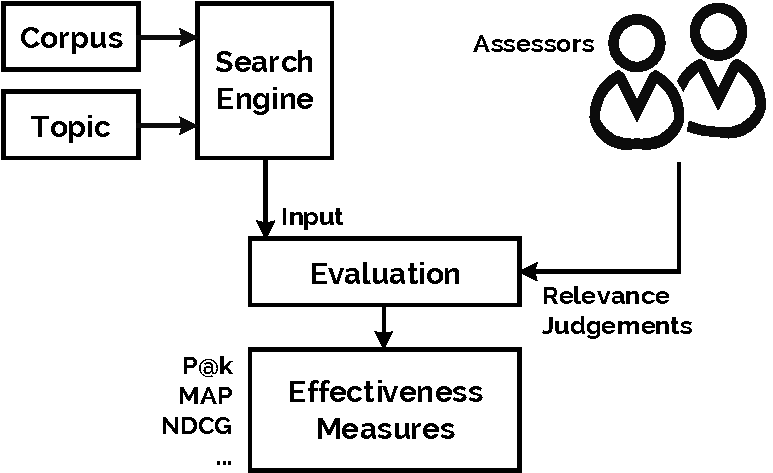
\includegraphics[width=\linewidth]{figures/cranfield.pdf}
% %     \caption{The Cranfield Paradigm. Document collections (corpora) and associated topics are created, and are then passed to assessors to judge the relevancy of documents against the provided topics. These judgements are then provided to researchers as \emph{relevance judgements}, which are then used to evaluate the performance of retrieval components with different \emph{effectiveness measures}, such as \boldmath{$P@k$}.}
% %     \label{fig:cranfield}
% %     \end{center}
% % \end{figure}
% %
% % \subsection{Why Simulation?}
% % A question that readers of this thesis may ask early on is: \emph{why use simulation?} Could the behaviours exhibited by human searchers instead be perhaps modelled through less computationally intensive means? This is a perfectly valid question to ask; indeed, the author tripped up when asked this question at the 1\textsuperscript{st} ACM CHIIR Doctoral Consortium.
% %
% % One of the potential criticisms of this work is: why simulate at all? Why not just plug everything into an equation, and solve it? \url{https://www.cise.ufl.edu/~fishwick/introsim/node2.html}
% %
% %
% % \section{Thesis Statement}
% %
% % - statement of fact: users are complex, and adapt their behaviour due to a variety of different factors, not limited to the ranked list of results presented to them.
% % - statement of fact: many of the models and measures that we use in IR do not assume this.
% % - one thing we do not consider much is stopping behaviour. by incorporating stopping behaviour into our models, we can provide better approximations of searcher behaviour
% %
% % - The statement of this thesis is that incorporating stopping level decision points into a user model will lead to more efficient searching, and better approximations of actual searcher behaviour
% %
% %
% % The statement of this thesis is that we can improve our understanding of the stopping behaviour of searchers through experimentation. This understanding can be further improved through the use of simulation.
% %
% %
% % \section{Overarching Research Questions}
% % From the introductory remarks, thesis statement and motivation as described above, we can now formulate the three main research questions that will be addressed in this thesis.
% %
% % \begin{itemize}
% %
% %     \item[]{\blueboxbold{RQ1} How can we improve upon and make \emph{more realistic models} of the~\gls{acr:iir} search process -- as a whole?}
% %
% %     \item[]{\blueboxbold{RQ2} How can we operationalise and subsequently implement more realistic stopping strategies for use within many of the commonly used~\gls{acr:ir} and~\gls{acr:iir} models and measures that are in use today?}
% %
% %     \item[]{\blueboxbold{RQ3} How do the real-world stopping behaviours of searchers vary under different contexts?}
% %
% % \end{itemize}
% %
% % Each of these research questions will be addressed in parts \blueboxbold{I} and \blueboxbold{II}.
% %
% % \section{Contributions}
% % The work undertaken towards completion of this thesis has led to a number of contributions to the field, many of which have been published in international conference proceedings. The following contributions have been made.
% %
% % \begin{itemize}
% %
% %     \item{An extensible simulator framework, called \emph{SimIIR}, that allows for full-session~\gls{acr:iir} simulation.}
% %
% %     \item{The introduction and evolution of the Complex Searcher Model, a full-session model of the~\gls{acr:iir} process. Note that this model does not attempt to model the brain; rather, it is a model of the overarching steps and decisions that a searcher makes during the search process. We do model state; this does not consider the brain, nor does the model consider other issues such as environmental factors.}
% %
% %     \item{A series of user studies that examine the effects of stopping behaviour on:}
% %
% %     \begin{itemize}
% %         \item{temporal delays;}
% %         \item{snippet lengths; and}
% %         \item{novelty and diversity of results.}
% %     \end{itemize}
% %
% % \end{itemize}
% %
% % \section{Outline}
% % This thesis is split into four logical parts, each of which constitutes a number of chapters.
% %
% % \begin{itemize}
% %
% %     \item{The remainder of \blueboxbold{Part I} provides background of the areas of Information Retrieval and simulation.}
% %
% %     \item{\blueboxbold{Part II} considers the approaches taken to develop the models of IIR further, introducing the Complex Searcher Model.}
% %
% %     \item{\blueboxbold{Part III} examines stopping behaviours, heuristics and strategies in detail, and how the behaviours of searchers is affected by various contexts.}
% %
% %     \item{Finally, \blueboxbold{Part IV} provides conclusions and future work.}
% %
% % \end{itemize}
%
% % --------------------------------
% % -------- NOV 28 BELOW ----------
% % --------------------------------
%
% % We live today in the so-called \emph{Information Age}, an era defined by the creation, transmission, management and \emph{retrieval} of information\footnote{\url{https://en.oxforddictionaries.com/definition/information_age} -- accessed November 26\textsuperscript{th}, 2017.}. With a steady incoming stream of e-mails, articles, and the near-instant reporting of events taking place all around the planet, one would be hard pressed to deny such a claim. Of course, none of this would be possible without the modern-day computer, a now ubiquitous device that can be found in a variety of different shapes and sizes (or \emph{form factors}). Nor would this be possible without the developments of the fundamental technologies that allow for communication between computers, such as the \emph{Internet} -- and associated technologies such as the~\gls{acr:www}~\citep{berners1994www}. Indeed, with technologies today allowing access to the Internet so commonplace, a recent \emph{IBM} technical report estimated that we generate something in the range of \emph{2.5 quintillion bytes} of information \emph{per day}\footnote{$2.5$ quintillion bytes = $2,500,000,000,000,000,000$ bytes, or $2,500,000$ terabytes.}.
% %
% % Sifting through such quantities of information has been a major research challenge, and the field of~\gls{acr:ir}~\citep{rijsbergen1979ir} has existed for several decades. Researchers began with the development
%
%
%
% % explanation of JumpStation~\citep{mcbryan1994taming_tools}
% %
% %
% % We live today in an age of information ubiquity. A constant barrage of e-mails, articles and webpages. A continuous stream of messages on social media platforms. Thanks to the development of the modern computer -- including its various form factors, like the smartphone -- the Internet and the subsequent technologies that have been developed on these key technological advancements -- such as the~\gls{acr:www}~\citep{berners1994www}, we now, according to an IBM technical report\footnote{\url{https://www-01.ibm.com/common/ssi/cgi-bin/ssialias?htmlfid=WRL12345USEN} -- last accessed November 23\textsuperscript{rd}, 2017.}, generate something in the range of 2.5 quintillion bytes\footnote{$2.5$ quintillion bytes = $2,500,000,000,000,000,000$ bytes} of information \emph{per day}.
% %
% % Since the invention of the World Wide Web at CERN in 1989, the \emph{de facto} approach to finding documents within the web of hyperlink documents has been the \emph{search engine}. Search engine technology, although analogous to web search, has been around for much longer -- and contemporary search engines that we use today on a daily basis such as \emph{Google} and \emph{Bing} are considered to offer an effective means of finding the proverbial needle in the haystack.
% %
% % \begin{quote}
% %     ``...but perhaps the key technology that took the Web from a useful supplement of current information practice to become the default communication medium is search.''
% %     \attrib{\citealp{wilson2010keyword_search}}
% % \end{quote}
% %
% % What, however, is the proverbial \emph{needle}? Much work has been undertaken in the field of~\gls{acr:iir} to ascertain and understand the needs of users of search engines. Searchers typically arrive at a search engine in an \emph{Anomalous State of Knowledge (ASK)}~\citep{belkin1980ask}, converting this need into some form of query formulation. The search engine then presents a series of documents to the searcher.
%
%
%
% % \begin{quote}
% %     ``When I first moved into the White House with President Bill Clinton in 1993, there were only 50 existing websites on the World Wide Web.''
% %     \attrib{Al Gore}
% % \end{quote}
%
% % - we live today in an information orientated world.
% % - we need to find information instantly.
% % - volume of information has increased massively.
% % - rate of information generation is remarkable.
% % - thanks to computers and the internet
% % - development of technologies lying upon internet infrastructure, such as the WWW have been key drivers in this development.
% % - 2.5 quintillion bytes of information created on a daily basis.
% %
% % - sifting through all of this information is obviously required.
% % - so the need to search has become paramount and key to our daily lives.
% % - finding the proverbial needle in a haystack is not easy - decades of work have led to this point.
% %
% % - originally, directory-based systems.
% % - but as information grew, so too did the need for search.
% %
% %     \begin{quote}
% %         \Large
% %         ``But perhaps the key technology that took the Web from a useful supplement of current information practice to become the default communication medium is search.''
% %         \attrib{Max Wilson}
% %     \end{quote}
% %
% % - indeed, what is the needle?
% % - searcher arrives in a anomouls state of knowledge.
% % - typically, a searcher will convert this need into some query formulation, and is presented with a series of documents.
% % - this is in essence how a retrieval system works.
% %
% % -
%
%
%
%
% % - as the volume of information that we create has increased, so too has our need to find the information that we need.
% %
% %
% % A searcher approaches an Information Retrieval (IR) system with a need for information derived from an ‘anomalous state of knowledge’ (Belkin et al., 1982). This need is typically transformed into a query statement, submitted to the system and a set of potentially relevant documents is retrieved and presented. The transformation of this need into a search expression, or query, is known as query formulation. Through such transformations and further interaction searchers can conduct Interactive IR (IIR), where they engage in dialogue with the IR system and it dynamically responds to their feedback (Borlund, 2003).
% %
% %
% % Arguably one of the most important developments of the mid-1990's was the introduction of the~\gls{acr:www}.
% %
% % Without it, there is no Google. Without it, there is no Facebook, or any of the other online services that keep the needs of billions satisfied (or perhaps even dissatisfied).
% %
% % The advancement of the~\gls{acr:www}~\citep{berners1994www}...
% %
% %
% % Computers advancement in our age
% % Since the advent of the World Wide Web in the mid-1990's, the amount of information that we generate as humans is estimated to be in the range of 2.5petabytes per day.
% %
% % the rate of information that we generate is remarkable.
% % we create 2.5 quintillion bytes of data per day.
% % 90 percent of all data created by man has been generated in the past few years.
% %
% % \footnote{https://www-01.ibm.com/common/ssi/cgi-bin/ssialias?htmlfid=WRL12345USEN}
% % \footnote{$2.5$ quintillion = $2,500,000,000,000,000,000$ bytes}